\documentclass[12pt]{report}
\usepackage[spanish]{babel}
\usepackage[utf8]{inputenc}
\usepackage{graphicx}
\usepackage{verbatim}
\usepackage{listings}
\usepackage{float}
\renewcommand*\thesection{\arabic{section}}

\begin{document}
	
	\begin{center}
		\textbf{Análisis de Algoritmos, Sem: 2018-1, 3CV1, Práctica 2, 09-2017}
		\newline
	\end{center}
	
	\begin{center}
		\begin{picture}(0,0) \put(-125,-55){
			\includegraphics[width=2.7cm]{../../IPNlogo.jpg}} 
		\end{picture}
		\LARGE Escuela Superior de Cómputo.\\
		Instituto Politécnico Nacional, México.\\
		\begin{picture}(0,0) \put(160,10){
			\includegraphics[width=2.7cm]{../../logoescom.png}} 
		\end{picture}
	\end{center}
	
	\begin{center}
		\Large Práctica 2: Funciones recursivas vs iterativas.\\
	\end{center}
	
	\begin{center}
		\textbf{Blancas Pérez Bryan Israel}\\
		orionmunecaycanica@gmail.com\\
	\end{center}
	
	
	\textbf{\large Resumen: }Demostrar de manera experimental y formal, el orden de complejidad de algoritmos (cuyo propósito es el mismo) implementados de dos formas distintas (algoritmo recursivo e iterativo), y comparar los resultados con el fin de identificar cuál de los algoritmos es más eficiente.\newline\\
	
	\textbf{\large Palabras Clave: } Algoritmo recursivo, algoritmo iterativo, complejidad computacional, cálculo formal del tiempo de ejecución.\\
	
	\section{Introducción}
		Un algoritmo iterativo es aquel que se ejecuta mediante ciclos iterativos, definidos o indefinidos, para llegar a la resolución del problema. Como opción a éstos, existen los algoritmos recursivos, los cuales usan la recursividad como herramienta para resolver el problema.\\ 
		La recursividad utiliza más recursos del sistema para su ejecución, es precisamente por ello que en ocasiones se tiene la creencia de que un algoritmo recursivo es siempre más lento que un algoritmo iterativo.\\
		Bajo la premisa de que todo algoritmo recursivo se puede expresar como un algoritmo iterativo y viceversa, en esta práctica mediante el análisis experimental y formal, se compararán ciertos algoritmos en sus dos implementaciones, con el fin de saber cuál es más eficiente dependiendo del problema.\\
		
	\section{Conceptos Básicos}
	\textbf{Recursividad.}\\
	La recursividad es la forma en la cual se especifica un proceso basado en su propia definición, es decir, construcción a partir del mismo tipo [1]. La técnica de solución de problemas "Divide y Vencerás", comúnmente nos lleva a la recursividad, debido a que se divide el problema en sub-problemas de la misma naturaleza, y por ende el mismo algoritmo para solucionar.\\ 
	Un ejemplo clásico del uso de la recursividad es el calculo del factorial de un número $n$. Ya que $n!$ se define como el producto de todos los números anteriores a $n$, se puede resolver el problema como $n(n-1)!=n(n-1)(n-2)!$ y así sucesivamente hasta llegar $0!=1$.\\
	
	\textbf{Iteración.}\\
	Iteración, según el DLE, significa repetir. En programación se interpreta como el acto de repetir un conjunto de instrucciones de manera definida o indefinida, con el fin de alcanzar el resultado deseado [2].
	
	
	
	\section{Experimentación y Resultados}	
	\textbf{Ejercicio 1.}\\
	
	Implementar la sucesión de Fibonacci mediante un algoritmo recursivo y mediante un algoritmo iterativo.\newline \\
	Pseudocódigo del algoritmo recursivo:
	\lstset{language=C, breaklines=true, basicstyle=\footnotesize}
	\lstset{numbers=left, numberstyle=\tiny, stepnumber=1, numbersep=10pt}
	\begin{lstlisting}
F(int n)
  if n < 2
    return n
  else
    return F(n-1)+F(n-2)
	\end{lstlisting}
	
	La función $F$, recibe como parámetro un entero n, que representa el n-ésimo termino de la sucesión. La condición de paro en este algoritmo, es cuando n < 2, ya que se llego al final de todos los términos. En caso contrario, se retorna a $F(n-1)+F(n-2)$, que se interpreta como la suma de los dos números anteriores al número actual. \\
	
	Pseudocódigo del algoritmo iterativo:
	\lstset{language=C, breaklines=true, basicstyle=\footnotesize}
	\lstset{numbers=left, numberstyle=\tiny, stepnumber=1, numbersep=10pt}
	\begin{lstlisting}
FI(int n)
  if n < 2 
    aux=1
  for i = 2 to i<=n do
    aux=a+b	
    a=b		
    b=aux
  return aux;
	\end{lstlisting}
	
	La función $FI$, recibe como parámetro un entero n, que representa el n-ésimo termino de la sucesión. El $for$ inicia en $2$, ya que previamente existe una condición para los primeros dos término de la sucesión, los cuales son iguales a 1. El ciclo calcula la suma de los dos números anteriores al número actual, y después actualiza los valores de las variables para el la siguiente iteración.\\
	
	Programa en ejecución\\
	\begin{figure}[H]
		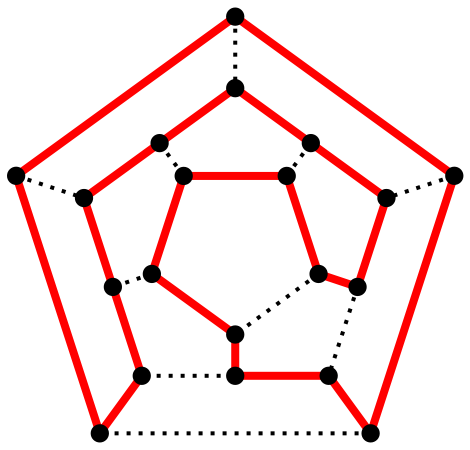
\includegraphics[width=4cm]{1.png}
		\centering
		\caption{Ejecución del programa 1.}
		\centering
	\end{figure}
	En la figura 1, se aprecia que el programa recibe como entrada el número el cual representa la pregunta ¿Cuál es el n-ésimo término de la sucesión de Fibonacci?. Como salida en la terminal, se muestra el número, primeramente el calculado con el algoritmo iterativo y después el calculado con el algoritmo recursivo.

	\begin{figure}[H]
		\includegraphics[width=4cm]{1_file.png}
		\centering
		\caption{Ejemplo de output en archivo del programa 1.}
		\centering
	\end{figure}
	En la figura 2, se muestra la salida del programa 1 en el archivo. La primer columna representa el n-ésimo término de la secesión de Fibonacci y la segunda columna representa el tiempo de ejecución (cont) que se requirió para terminar exitosamente el programa.\\
		
	Gráfica de resultado algoritmo recursivo.\\
		\begin{figure}[H]
			\includegraphics[height=10cm]{grafica1_recursivo.png}
			\centering
			\caption{Gráfica del ejecicio 1 recursivo.}
			\centering
		\end{figure}
	En la figura 3, se muestra la gráfica $T(n) \ vs \ n$, en la que los puntos marcados corresponden a los datos obtenidos en el archivo de salida del ejercicio 1. Como es apreciable, el orden de complejidad del algoritmo recursivo, para calcular el n-ésimo término de la sucesión de Fibonacci tiene orden exponencial.\newpage
	
	Gráfica de resultado algoritmo recursivo.\\
	\begin{figure}[H]
		\includegraphics[height=9cm]{grafica1_iterativo.png}
		\centering
		\caption{Gráfica del ejecicio 1 recursivo.}
		\centering
	\end{figure}
	En la figura 4, se muestra la gráfica $T(n) \ vs \ n$, en la que los puntos marcados corresponden a los datos obtenidos en el archivo de salida del ejercicio 1. Como es apreciable, el orden de complejidad del algoritmo iterativo, para calcular el n-ésimo término de la sucesión de Fibonacci tiene orden lineal.\newpage
	
	\textbf{Comprobación del orden de complejidad del algoritmo iterativo.} \\
	
\lstset{language=C, breaklines=true, basicstyle=\footnotesize}
\lstset{numbers=left, numberstyle=\tiny, stepnumber=1, numbersep=10pt}
\begin{lstlisting}
FI(int n)
  if n < 2 
    aux=1
  for i = 2 to i<=n do
    aux=a+b	
    a=b		
    b=aux
  return aux;
\end{lstlisting}

\begin{table}[htbp]
	\begin{center}
		\begin{tabular}{|l|l|l|}
			\hline
			\multicolumn{3}{|c|}{Análisis del Algoritmo} \\ 
			\hline
			\textbf{Línea de Código} & \textbf{Tiempo Ejecución} & \textbf{Número de Ejecuciones}\\
			\hline
			2 & C1 & $1$ \\ \hline
			3 & C2 & $1$ \\ \hline
			4 & C3 & $n$ \\ \hline
			5 & C4 & $(n-1)$ \\ \hline
			6 & C5 & $(n-1)$ \\ \hline
			7 & C6 & $(n-1)$ \\ \hline
			8 & C7 & $1$ \\ \hline
		\end{tabular}
		\caption{Análisis del algoritmo.}
		\label{tabla:analisis}
	\end{center}
\end{table}
Encontrando el orden de complejidad.\\
$T(n)= C1+C2+C3n+C4(n-1)+C5(n-1)+C6(n-1)+C7.$\\
$T(n)= (C3+C4+C5+C6)n+C1+C2-C4-C5-C6+C7.$\\
$T(n)=An+B.$\\

$Por \ lo \ tanto \ \ \ T(n) \ \epsilon \ \theta (n).$\newpage
	
	\textbf{Ejercicio 2.}\\
	
	Implementar el algoritmo dado para calcular la suma de los primeros $n$ cubos , e implementar otro algoritmo pero de manera iterativa.\newline \\
	Pseudocódigo del algoritmo recursivo del ejercicio 2:
	\lstset{language=C, breaklines=true, basicstyle=\footnotesize}
	\lstset{numbers=left, numberstyle=\tiny, stepnumber=1, numbersep=10pt}
	\begin{lstlisting}
S (int n)
  if n == 1
    return 1
  else
    return S(n-1) + (n * n * n)
	\end{lstlisting}
	
	La función $S$, recibe como parámetro un número entero positivo. La condición de paro es cuando el número es igual a uno, en caso contrario, se retornará la función $S(n-1)$, es decir el número que continúa en orden descendente, más el número actual elevado al cubo.\\
	
	Pseudocódigo del algoritmo iterativo del ejercicio 2:
	\lstset{language=C, breaklines=true, basicstyle=\footnotesize}
	\lstset{numbers=left, numberstyle=\tiny, stepnumber=1, numbersep=10pt}
	\begin{lstlisting}
SI(int n)
  for i = 1 to i <= n do
	aux += i * i * i
return aux;
	\end{lstlisting}
	
	La función $SI$, recibe como parámetro un número entero positivo. El algoritmo inicia un $for$, hasta que i sea igual a el número dado. En cada iteración, se guarda en una variable auxiliar la suma de el número elevado al cubo más lo que había anteriormente.\\
	
	Programa en ejecución\\
	\begin{figure}[H]
		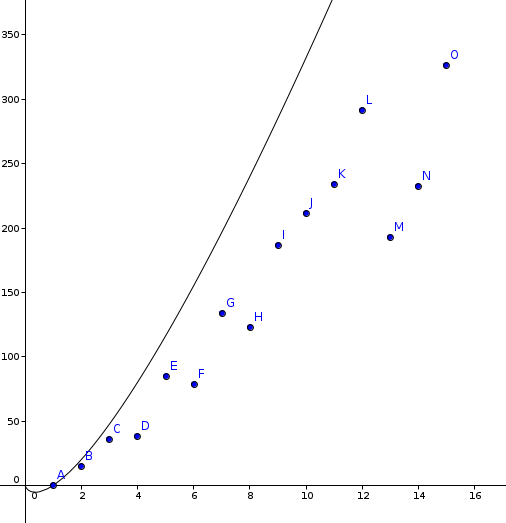
\includegraphics[width=4cm]{2.png}
		\centering
		\caption{Ejecución del programa 2.}
		\centering
	\end{figure}
	En la figura 5, se muestra que el programa recibe como entrada el número del cual se quiere saber cuanto es la suba de los n primeros números al cubo. Como salida en la terminal, se muestra al cálculo con ambos algoritmos.
	\begin{figure}[H]
		\includegraphics[height=4cm]{2_file.png}
		\centering
		\caption{Ejemplo de output en archivo del programa 2.}
		\centering
	\end{figure}
	En la figura 4, se muestra la salida del programa 2 en el archivo. La primera columnas es el número $n$ y la segunda columna representa el tiempo de ejecución (cont) que se requirió para calcular la suma.\\
	
	
	Gráfica de resultado.\\
	\begin{figure}[H]
		\includegraphics[height=6cm]{grafica2_recursivo.png}
		\centering
		\caption{Gráfica 1 del ejercicio 2.}
		\centering
	\end{figure}
	En la figura 7, se muestra la gráfica $T(n) \ vs \ n$, en la que los puntos marcados corresponden a los datos obtenidos en el archivo de la ejecución del programa 2. La práctica pide proponer una función $g(n) $ tal que $T(n) \ \epsilon \ O(g(n))$, en este caso $g(n)=3x$\\
	
	\begin{figure}[H]
		\includegraphics[height=6cm]{grafica2_iterativo.png}
		\centering
		\caption{Gráfica 2 del ejercicio 2.}
		\centering
	\end{figure}
	En la figura 8, se muestra la gráfica $T(n) \ vs \ n$, en la que los puntos marcados corresponden a los datos obtenidos en el archivo de salida del ejercicio 2 iterativo.  La práctica pide proponer una función $g(n) $ tal que $T(n) \ \epsilon \ O(g(n))$, en este caso $g(n)=3x$.\newpage
	
	\textbf{Comprobación del orden de complejidad del algoritmo iterativo.} \\
	
	\lstset{language=C, breaklines=true, basicstyle=\footnotesize}
	\lstset{numbers=left, numberstyle=\tiny, stepnumber=1, numbersep=10pt}
	\begin{lstlisting}
SI(int n)
  for i = 1 to i <= n do
    aux += i * i * i
  return aux;
	\end{lstlisting}
	
	\begin{table}[htbp]
		\begin{center}
			\begin{tabular}{|l|l|l|}
				\hline
				\multicolumn{3}{|c|}{Análisis del Algoritmo} \\ 
				\hline
				\textbf{Línea de Código} & \textbf{Tiempo Ejecución} & \textbf{Número de Ejecuciones}\\
				\hline
				2 & C1 & $n+1$ \\ \hline
				3 & C2 & $n$ \\ \hline
				4 & C3 & $1$ \\ \hline
			\end{tabular}
			\caption{Análisis del algoritmo.}
			\label{tabla:analisis2}
		\end{center}
	\end{table}
	Encontrando el orden de complejidad.\\
	$T(n)= C1(n-1)+C2n+C3.$\\
	$T(n)= (C1+C2)n+C3-C1.$\\
	$T(n)=An+B.$\\
	$Por \ lo \ tanto \ \ \ T(n) \ \epsilon \ \theta (n).$\newpage
	
	\textbf{Comprobación de complejidad del algoritmo recursivo.} \\
	\lstset{language=C, breaklines=true, basicstyle=\footnotesize}
	\lstset{numbers=left, numberstyle=\tiny, stepnumber=1, numbersep=10pt}
	\begin{lstlisting}
S (int n)
  if n == 1
    return 1
  else
    return S(n-1) + (n * n * n)
	\end{lstlisting}

	Encontrando el orden de complejidad.\\		
	$Se \ tiene \ que$\\
	
	 $f(n) = \left \{ \begin{array}{c} 1 \ si \ n=1 \\ s(n-1)+n^{3} \ si \ n \ > \ 1 \end{array}\right.$\\
	 
	Sea M(n) el número de sumas para f(n).\\
	
	 $M(n) = \left \{ \begin{array}{c} 0 \ si \ n=1 \\ M(n-1)+1 \ si \ n \ > \ 1 \end{array}\right.$\\
	 
	 Entonces:\\
	$M(n)=M(n-1)+1$\\
	$M(n)=M(n-2)+2$\\
	i-ésimo término.\\
	$M(n)=M(n-i)+i$\\
	cuando i=n.\\
	$M(n)=M(0)+n$\\
	$M(n)=1+n$\\
	
	$Por \ lo \ tanto \ \ \ M(n) \ \epsilon \ \theta (n).$\newpage
	
	\section{Conclusiones}
	Esta práctica para mi es muy útil para darme cuenta de que no hay un algoritmo que sea mejor que otro simplemente por ser de un tipo. En el desarrollo de la práctica se puede apreciar que hay algoritmos los cuales tiene el mismo orden de complejidad computacional, tanto en su implementación recursiva como en la iterativa.\\
	Uno de los problemas que tuve al desarrollar la práctica, es que al graficar el output del algoritmo recursivo de Fibonacci, me graficaba una función lineal, lo cual era incorrecto, ya que como nos había dicho el profesor previamente, el algoritmo recursivo de fibonacci tiene orden de complejidad exponencial. Este problema lo solucioné cambiando el algoritmo, debido a que la primera versión de éste que había hecho, estaba mal implementada.
	
	
	\section{Anexo}
	
	Resolver el siguiente problema.\\
	
	Calcular el orden de complejidad de algoritmo de la burbuja (BubbleSort).\\
	
	\lstset{language=vhdl, breaklines=true, basicstyle=\footnotesize}
	\lstset{numbers=left, numberstyle=\tiny, stepnumber=1, numbersep=10pt}
	\begin{lstlisting}
BubbleSort(A)
  for i = 1 to i <= A.length-1 do
    for j = A.length downto j >= i+1
      if A[j] < A[j-1]
        exchange A[j] with A[j-1]
	\end{lstlisting}
	
	Encontrando el orden de complejidad.\\
	
	\begin{table}[htbp]
		\begin{center}
			\begin{tabular}{|l|l|l|}
				\hline
				\multicolumn{3}{|c|}{Análisis del Algoritmo} \\ 
				\hline
				\textbf{Línea de Código} & \textbf{Tiempo Ejecución} & \textbf{Número de Ejecuciones}\\
				\hline
				2 & C1 & $n$ \\ \hline
				3 & C2 & $\sum_{1}^{n}(ti)$ \\ \hline
				4 & C3 & $\sum_{1}^{n}(ti-1)$ \\ \hline
				5 & C4 & $\sum_{1}^{n}(ti-1)$ \\ \hline
			\end{tabular}
			\caption{Análisis del algoritmo.}
			\label{tabla:analisis3}
		\end{center}
	\end{table}\newpage

Sea $t_{i}$ el número de veces que se ejecuta esa línea de código. Entonces.
$T(n)=C1(n)+C2\sum_{1}^{n}(ti)+(C3+C4)\sum_{1}^{n}(ti-1).$\\

Pero.\\

\begin{table}[htbp]
	\begin{center}
		\begin{tabular}{|l|l|l|}
			\hline
			\multicolumn{3}{|c|}{Encontrando ti} \\ 
			\hline
			\textbf{i} & \textbf{i+1 $\leq$ j $\leq$ n} & \textbf{ti}\\
			\hline
			1 & $2 \leq j \leq n$ & $n-1$ \\ \hline
			2 & $3 \leq j \leq n$ & $n-2$ \\ \hline
			3 & $4 \leq j \leq n$ & $n-3$ \\ \hline
			... & ... & ... \\ \hline
			i & $i \leq j \leq n$ & $n-i$ \\ \hline
		\end{tabular}
		\caption{Encontrando ti}
	\end{center}
\end{table}

Entonces.\\
$T(n)=C1(n)+C2\sum_{1}^{n}(n-i)+(C3+C4)\sum_{1}^{n}(n-i-1).$\\
$T(n)=C1(n)+C2(n^{2}-\frac{n(n+1)}{2})+(C3+C4)(n^{2}-\frac{n(n+1)}{2}-n).$\\
$T(n)=(C2+C3+C4)\frac{n^{2}}{2}+(C1-\frac{C2}{2}-\frac{3(C3+C4)}{2})n.$\\
$T(n)=An^{2}+Bn.$\\

$ por \ lo \ tanto \ \ \ T(n) \ \epsilon \ \theta (n^{2})$
	
	\section{Bibliografía}
	
	[1] es.wikipedia,org/wiki/Recursión.\\
	
	[2] es.wikipedio.org/wiki/Iteración.
	
\end{document}